% Figure: the three cases of the locality lemma for the first coordinate
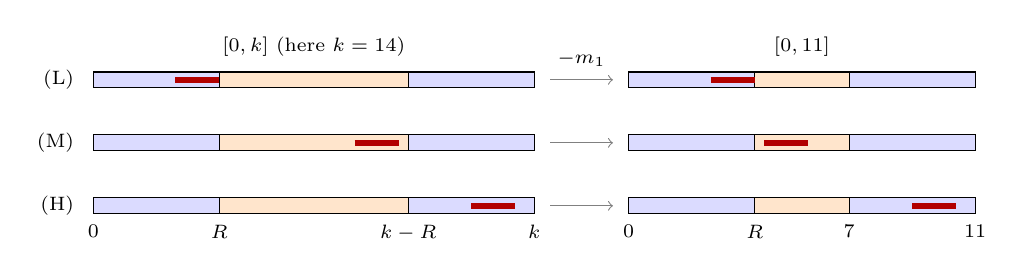
\begin{tikzpicture}[x=0.4cm,y=0.5cm,font=\scriptsize]
  \foreach \row/\lab/\a/\b/\aa/\bb in {0/(L)/2.6/4.0/2.6/4.0, -1.6/(M)/8.3/9.7/4.3/5.7, -3.2/(H)/12.0/13.4/9.0/10.4} {
    \begin{scope}[shift={(0,\row)}]
      \node[left] at (-0.3,0) {\lab};
      \fill[blue!14] (0,-0.2) rectangle (4,0.2); \fill[orange!20] (4,-0.2) rectangle (10,0.2); \fill[blue!14] (10,-0.2) rectangle (14,0.2);
      \draw (0,-0.2) rectangle (14,0.2); \draw (4,-0.2)--(4,0.2) (10,-0.2)--(10,0.2);
      \draw[line width=2pt,red!70!black] (\a,0) -- (\b,0);
      \begin{scope}[shift={(17,0)}]
        \fill[blue!14] (0,-0.2) rectangle (4,0.2); \fill[orange!20] (4,-0.2) rectangle (7,0.2); \fill[blue!14] (7,-0.2) rectangle (11,0.2);
        \draw (0,-0.2) rectangle (11,0.2); \draw (4,-0.2)--(4,0.2) (7,-0.2)--(7,0.2);
        \draw[line width=2pt,red!70!black] (\aa,0) -- (\bb,0);
      \end{scope}
      \draw[->,gray] (14.5,0) -- (16.5,0);
    \end{scope}}
  \node[above] at (7,0.35) {$[0,k]$ (here $k=14$)}; \node[above] at (22.5,0.35) {$[0,11]$};
  \node[above] at (15.5,0.1) {$-m_1$};
  \foreach \x/\l in {0/0,4/R,10/k-R,14/k} \node[below] at (\x,-3.45) {$\l$};
  \foreach \x/\l in {17/0,21/R,24/7,28/11} \node[below] at (\x,-3.45) {$\l$};
\end{tikzpicture}
